\begin{frame}
    \frametitle{
        Numerical Quadrature~\cite[p.~397]{salgado_classical_2022}
    }

    Let
    \begin{math}
        f\in
        \continuous
    \end{math}.
    We seek calculate an approximation of
    \begin{equation*}
        I^{\left(a,b\right)}
        \left[f\right]\coloneqq
        \int_{a}^{b}
        f\left(x\right)
        \dl x.
    \end{equation*}

    Suppose that
    \begin{math}
        g\in
        \continuous
    \end{math},
    whose antiderivative is simply obtained, and
    \begin{math}
        {\left\|f-g\right\|}_{\infty}<
        \varepsilon
    \end{math}.
    Then,
    \begin{equation*}
        \left|
        \int_{a}^{b}
        f\left(x\right)
        \dl x-
        \int\limits_{a}^{b}
        g\left(x\right)
        \dl x
        \right|\leq
        \varepsilon
        \left(b-a\right).
    \end{equation*}

    \begin{definition}[Nodal set]
        Let
        \begin{math}
            \interval\subset
            \mathbb{R}
        \end{math}.
        $X$ is called a \emph{nodal set} of size $n+1\in\mathbb{N}$
        iff
        \begin{math}
            \nodalset\subset
            \interval
        \end{math}
        is a set of distinct elements.
        The elements of $X$, $x_{i}$ are called \emph{nodes}.
    \end{definition}

    \begin{definition}[Interpolating polynomial]
        Suppose that
        \begin{math}
            \nodalset\subset
            \interval
        \end{math}
        is a nodal set and
        \begin{math}
            f\colon
            \interval\to
            \mathbb{R}
        \end{math}
        is a function.
        The function
        \begin{math}
            I\colon
            \interval\to
            \mathbb{R}
        \end{math}
        is called an \emph{interpolant of} $f$ subordinate to $X$ iff
        \begin{math}
            \forall i=0,\dotsc,n:
            I\left(x_{i}\right)=
            f\left(x_{i}\right)
        \end{math},
        we write
        \begin{math}
            I\left(X\right)=
            f\left(X\right)
        \end{math}.
    \end{definition}
\end{frame}

\begin{frame}
    % TODO: Interpolant
    % \begin{definition}[Interpolant]
    %     Suppose
    %     \begin{math}
    %         Y=
    %         {\left\{y_{i}\right\}}_{i=0}^{n}\subset
    %         \mathbb{R}
    %     \end{math}
    %     is a set of not necessarily distinct points.
    %     Define the set of ordered pairs
    %     \begin{equation*}
    %         O=
    %         \left\{
    %         \left(x_{i},y_{i}\right)\mid
    %         x_{i}\in X,
    %         y_{i}\in Y,
    %         \forall i=0,\dotsc,n
    %         \right\}.
    %     \end{equation*}
    %     We say that $I$ is an \emph{interpolant} of $O$ iff
    %     \begin{math}
    %         \forall i=0,\dotsc,n:
    %         I\left(x_{i}\right)=
    %         y_{i}
    %     \end{math},
    %     we write
    %     \begin{math}
    %         I\left(X\right)=
    %         Y
    %     \end{math}.
    %     If the interpolant $I$ is a polynomial, it is called an
    %     \emph{interpolating polynomial}.
    % \end{definition}

    \begin{theorem}[existence and uniqueness]
        Suppose that
        \begin{math}
            \nodalset\subset
            \interval
        \end{math}
        is a nodal set
        and
        \begin{math}
            Y=
            {\left\{
            y_{i}
            \right\}}_{i=0}^{n}\subset
            \mathbb{R}
        \end{math}.
        There is a unique polynomial $p\in\mathbb{P}_{n}$ with the
        property that $p\left(X\right)=Y$.
    \end{theorem}

    % TODO: Interpolation operator
    % \begin{definition}[Interpolation operator]
    %     Suppose that
    %     \begin{math}
    %         \nodalset\subset
    %         \interval
    %     \end{math}.
    %     The \emph{interpolation operation} subordinate to $X$,
    %     denoted
    %     \begin{equation*}
    %         \mathcal{I}_{X}\colon
    %         \continuous\to
    %         \mathbb{P}_{n},
    %     \end{equation*}
    %     is defined as follows: for
    %     \begin{math}
    %         f\in
    %         \continuous
    %     \end{math},
    %     \begin{math}
    %         \mathcal{I}_{X}
    %         \left[f\right]\in
    %         \mathbb{P}_{n}
    %     \end{math}
    %     is the unique interpolating polynomial satisfying
    %     \begin{math}
    %         \mathcal{I}_{X}
    %         \left[f\right]
    %         \left(X\right)=
    %         f\left(X\right)
    %     \end{math}.
    % \end{definition}

    \begin{definition}[Lagrange nodal basis]
        Suppose that
        \begin{math}
            \nodalset\subset
            \interval
        \end{math}
        is a nodal set.
        The \emph{Lagrange nodal basis} subordinate to $X$ is the set
        of polynomials
        \begin{math}
            \mathcal{L}_{X}=
            {\left\{
            L_{\ell}
            \right\}}_{\ell=0}^{n}\subset
            \mathbb{P}_{n}
        \end{math}
        defined via
        \begin{equation*}
            L_{\ell}
            \left(x\right)=
            \prod\limits_{\substack{i=0\\i\neq\ell}}^{n}
            \dfrac{x-x_{i}}{x_{\ell}-x_{i}}.
        \end{equation*}
    \end{definition}

    % TODO: Properties of \mathcal{L}_{X}

    % TODO: interpolating polynomial

    \begin{definition}[Lagrange interpolating polynomial]
        Suppose that
        \begin{math}
            \nodalset\subset
            \interval
        \end{math}
        is a nodal set,
        \begin{math}
            \mathcal{L}_{X}=
            {\left\{L_{i}\right\}}_{i=0}^{n}
            \subset
            \mathbb{P}_{n}
        \end{math}
        is the Lagrange nodal basis subordinate to $X$, and
        \begin{math}
            f\colon
            \interval\to
            \mathbb{R}
        \end{math}.
        The \emph{Lagrange interpolating polynomial} of the function
        $f$, subordinate to the nodal set $X$, is the polynomial
        \begin{equation*}
            p\left(x\right)=
            \sum_{i=0}^{n}
            f\left(x_{i}\right)
            L_{i}\left(x\right)\in
            \mathbb{P}_{n}.
        \end{equation*}
    \end{definition}
\end{frame}

\begin{frame}
    Suppose that
    \begin{math}
        \nodalset\subset
        \interval
    \end{math}
    is a nodal set and $p\in\mathbb{P}_{n}$ is the unique Lagrange
    interpolating polynomial of $f$ subordinate to $X$.
    Then
    \begin{equation*}
        \forall i=0,\dotsc,n:
        f\left(x_{i}\right)=
        p\left(x_{i}\right)
    \end{equation*}
    and
    \begin{equation*}
        \forall x\in
        \interval:
        f\left(x\right)=
        p\left(x\right)+
        E\left(x\right),
    \end{equation*}
    where $E$ is an expression of the interpolation error.
    Then
    \begin{equation*}
        \int_{a}^{b}
        f\left(x\right)
        \dl x=
        \int_{a}^{b}
        p\left(x\right)
        \dl x+
        \int_{a}^{b}
        E\left(x\right)
        \dl x.
    \end{equation*}
    But
    \begin{equation*}
        \int_{a}^{b}
        p\left(x\right)
        \dl x=
        \int_{a}^{b}
        \sum_{i=0}^{n}
        f\left(x_{i}\right)
        L_{i}\left(x\right)=
        \sum_{i=0}^{n}
        f\left(x_{i}\right)
        \int_{a}^{b}
        L_{i}\left(x\right)=
        \sum_{i=0}^{n}
        f\left(x_{i}\right)
        \beta_{i},
    \end{equation*}
    where $L_{i}\in\mathbb{P}_{n}$ is the $i$th Lagrange nodal basis
    element and $\beta_{i}$ is its definite integral:
    \begin{equation*}
        \beta_{i}=
        \int_{a}^{b}
        L_{i}\left(x\right)
        \dl x.
    \end{equation*}
    The expression
    \begin{math}
        \sum_{i=0}^{n}
        f\left(x_{i}\right)
        \beta_{i}
    \end{math}
    is a typical numerical integration formula
    \begin{equation*}
        \left|
        \int_{a}^{b}
        f\left(x\right)
        \dl x-
        \sum_{i=0}^{n}
        f\left(x_{i}\right)
        \beta_{i}
        \right|=
        \left|
        \int_{a}^{b}
        E\left(x\right)
        \dl x
        \right|\leq
        \int_{a}^{b}
        \left|
        E\left(x\right)
        \right|
        \dl x.
    \end{equation*}
\end{frame}

\begin{frame}

    \begin{definition}[Quadrature rule]
        Suppose that $n,r\in\mathbb{N}_{0}$,
        $w$ is a weight function on
        \begin{math}
            \interval\subset
            \mathbb{R}
        \end{math},
        $h=b-a>0$, and
        \begin{math}
            f\in
            C^{r}\left(
            \interval
            \right)
        \end{math}.
        The expression
        \begin{equation*}
            Q^{\left(a,b\right)}_{w,r}
            \left[f\right]=
            \sum_{i=0}^{r}
            \sum_{j=0}^{n}
            \beta_{i,j}
            f^{\left(i\right)}
            \left(x_{j}\right)=
            \sum_{j=0}^{n}
            \left(
            \beta_{0,j}
            f\left(x_{j}\right)+
            \beta_{1,j}
            f^{\prime}
            \left(x_{j}\right)+
            \cdots+
            \beta_{r,j}
            f^{\left(r\right)}
            \left(x_{j}\right)
            \right),
        \end{equation*}
        where
        \begin{math}
            \forall i\in
            \left\{0,\dotsc,r\right\}:
            \forall j\in
            \left\{0,\dotsc,n\right\}:
            \beta_{i,j}=
            h^{i+1}
            \widehat{\beta_{i,j}}
        \end{math}
        and
        \begin{math}
            \forall j\in
            \left\{0,\dotsc,n\right\}:
            x_{j}=
            a+
            h\cdot
            \widehat{x}_{j}
        \end{math}.
    \end{definition}
\end{frame}

\begin{frame}
    \begin{theorem}[Error estimate]
        Suppose that $n\in\mathbb{N}_{0}$, $w$ is a weight function
        on
        \begin{math}
            \interval\subset
            \mathbb{R}
        \end{math}.
        \begin{math}
            f\in C^{n+1}
            \left(
            \interval
            \right)
        \end{math},
        and
        \begin{math}
            X=
            \left\{x_{i}\right\}_{i=0}^{n}\subset
            \interval
        \end{math}.
    \end{theorem}

    \begin{equation*}
        Q^{\left(a,b\right)}_{w}
        \interval=
        \sum_{j=0}^{n}
        \beta_{j}
        f\left(x_{j}\right).
    \end{equation*}

    Simple quadrature rule.

    \begin{definition}[Closed Newton-Cotes quadrature rule]
        Suppose that $w$ is a weight function on
        \begin{math}
            \interval\subset
            \mathbb{R}
        \end{math}
        and $n\in\mathbb{N}$.
        Set $h=b-a>0$ and $\hslash=\frac{h}{n}$
    \end{definition}

    \begin{table}[ht!]
        \centering
        \begin{tabular}{ccccc}
            n & rule                                                          & $\widehat{x}_{j}$  & $\widehat{\beta}_{j}$
              & Error Formula                                                                                                                   \\
            1 & Trapezoidal                                                   & $0,1$              & $\dfrac{1}{2}, \dfrac{1}{2}$
              & $-\dfrac{1}{12}\hslash^{3}f^{\left(2\right)}\left(\xi\right)$                                                                   \\
            2 & Simpson's                                                     & $0,\dfrac{1}{2},1$ & $\dfrac{1}{6}, \dfrac{4}{6}, \dfrac{1}{6}$
              & $-\dfrac{1}{90}\hslash^{5}f^{\left(4\right)}\left(\xi\right)$
        \end{tabular}
    \end{table}

    \begin{theorem}[Error estimate]
        Let
        \begin{math}
            \interval\subset
            \mathbb{R}
        \end{math}.
        Suppose that is a closed Newton-Cotes quadrature rule of
        order $n\in\mathbb{N}$.
        Then, the order of quadrature rule is consistent of order at
        least $n$.
        Moreover, if $f\in C^{n+1}\left(\interval\right)$, then
        \begin{equation*}
            \left|
            E_{Q_{n}}
            \left[f\right]
            \right|\leq
            C
            h^{n+2}
            {\left\|f^{\left(n+1\right)}\right\|}_{\infty}
        \end{equation*}
    \end{theorem}
\end{frame}

\begin{frame}
    \begin{theorem}[Integral Mean Value Theorem]
        Let $a<b$,
        \begin{math}
            f\in
            \continuous
        \end{math},
        and
        \begin{math}
            g\in
            \mathcal{R}\left(a,b\right)
        \end{math}.
        Furthermore, suppose that $g\left(x\right)\geq0$ for all
        $x\in\interval$.
        Then, there exists $\xi\in\interval$ such that
        \begin{equation*}
            \int_{a}^{b}
            f\left(x\right)
            g\left(x\right)
            \dl x=
            f\left(\xi\right)
            \int_{a}^{b}
            g\left(x\right)
            \dl x.
        \end{equation*}

        Thus, if
        \begin{math}
            \forall x\in
            \interval:
            g\left(x\right)=
            1
        \end{math},
        there exists a point $\xi\in\interval$ such that
        \begin{equation*}
            f\left(\xi\right)=
            \dfrac{1}{b-a}
            \int_{a}^{b}
            f
        \end{equation*}
    \end{theorem}

    \begin{definition}
        Average concentration on
        \begin{math}
            \left[
                x-\frac{1}{2}h,
                +x\frac{1}{2}h
                \right]
        \end{math}.

        \begin{equation*}
            \overline{u}
            \left(x,t\right)=
            \dfrac{1}{h}
            \int_{x-\frac{1}{2}h}^{x+\frac{1}{2}h}
            u\left(s,t\right)
            \dl s.
        \end{equation*}
    \end{definition}
\end{frame}

\begin{frame}

    \begin{theorem}[Mass conservation law]
        If $u\left(x,t\right)$ is a concentration and
        \begin{equation*}
            M\left(t\right)\coloneqq
            \int_{0}^{1}
            u\left(x,t\right)
            \dl x
        \end{equation*}
        represents the mass in $\left[0,1\right]$ at time $t$, then
        $M$ is a conserved quantity.
    \end{theorem}

    \begin{proof}
        \begin{align*}
            \diff{M\left(t\right)}{t} & =
            \int_{0}^{1}
            u_{t}\left(x,t\right)
            \dl x=
            \int_{0}^{1}
            \left(
            -au_{x}\left(x,t\right)+
            du_{xx}\left(x,t\right)
            \right)\dl x                  \\
                                      & =
            -a\left(
            u\left(1,t\right)-
            u\left(0,t\right)
            \right)+
            d\left(
            u_{x}\left(1,t\right)-
            u_{x}\left(0,t\right)
            \right)=0.
        \end{align*}
    \end{proof}
\end{frame}

\begin{frame}
    \begin{figure}[ht!]
        \centering
        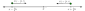
\includegraphics[width=.4\paperwidth]{deduction}
    \end{figure}

    \begin{definition}[Advection equation]
        \begin{equation*}
            u_{t}+du_{x}=0.
        \end{equation*}
    \end{definition}

    \begin{definition}[Diffusion equation]
        \begin{equation*}
            u_{t}=
            du_{xx}.
        \end{equation*}
    \end{definition}

    Let $h>0$, $h<<1$
\end{frame}